


\begin{frame}{Current Directions}
  \begin{center}
    \Large PETSc on GPUs and MIC: \\[1em] Current Directions \\[1em]
    %\includegraphics[width=0.5\textwidth]{figures/xkcd-pointers}
  \end{center}
\end{frame}


% cuBLAS and friends
\begin{frame}[fragile]
\frametitle{Current: CUDA}
  \begin{block}{Split CUDA-buffers from CUSP}
  \begin{itemize}
   \item Vector operations by cuBLAS
   \item MatMult by different packages
   \item CUSP (and others) provides add-on functionality
  \end{itemize}
  \end{block}
  
  \begin{center}
   \includegraphics[width=0.6\textwidth]{figures/cuda-arch}
  \end{center}

  %\pause 
  \begin{block}{More CUSP Functionality in PETSc}
   \begin{itemize}
    \item Relaxations (Gauss-Seidel, SOR)
    \item Polynomial preconditioners
    \item Approximate inverses
   \end{itemize}
  \end{block}

\end{frame}


% ViennaCL: CUDA, OpenCL, OpenMP
\begin{frame}[fragile]
\frametitle{Current: PETSc + ViennaCL}

\begin{minipage}{0.58\textwidth}
  \begin{block}{ViennaCL}
  \begin{itemize}
   \item CUDA, OpenCL, OpenMP backends
   \item Backend switch at \textbf{runtime}
   \item Only OpenCL exposed in PETSc
   \item Focus on shared memory machines
  \end{itemize}
  \end{block}
\end{minipage}
\begin{minipage}{0.4\textwidth}
   \includegraphics[width=0.999\textwidth]{figures/ViennaCL-arch}
\end{minipage}

  %\pause
  \vspace*{0.3cm}
  \begin{block}{Recent Advances}
  \begin{itemize}
   \item Pipelined Krylov solvers
   \item Fast sparse matrix-vector products
   \item Fast sparse matrix-matrix products
   \item Fine-grained algebraic multigrid
   \item Fine-grained parallel ILU
  \end{itemize}
  \end{block}

\end{frame}


\begin{frame}[fragile]
\frametitle{Current: PETSc + ViennaCL}

  \begin{block}{Current Use of ViennaCL in PETSc}
  \begin{itemize}
   \item 
  \begin{lstlisting}
 $> ./ex12 -vec_type viennacl -mat_type aijviennacl ...
  \end{lstlisting}
   \item Executes on OpenCL device
  \end{itemize}
  \end{block}

  %\pause
  
  \begin{block}{New Use of ViennaCL in PETSc}
  \begin{itemize}
   \item 
  \begin{lstlisting}
 $> ./ex12 -vec_type viennacl -mat_type aijviennacl
           -viennacl_backend openmp ...
  \end{lstlisting}
  \end{itemize}
  \end{block}

  %\pause
  
  \begin{block}{Pros and Cons}
  \begin{itemize}
   \item Use CPU + GPU simultaneously
   %\item Good PETSc performance on Theta, Aurora, Summit, ...
   \item Non-intrusive, use plugin-mechanism
   \item Non-optimal in strong-scaling limit
   \item Gather experiences for best long-term solution
  \end{itemize}
  \end{block}

\end{frame}


% Pipelined iterative solvers
\begin{frame}{Upcoming PETSc+ViennaCL Features}
  \begin{block}{Pipelined CG Method, Exec. Time per Iteration}
  \vspace*{-.5cm}
   \begin{center}
    \includegraphics[width=0.85\textwidth]{figures/cg}
   \end{center}
  \end{block}
\end{frame}

% SpMV
\begin{frame}{Upcoming PETSc+ViennaCL Features}
  \begin{block}{Sparse Matrix-Vector Multiplication}
   \begin{center}
    \includegraphics[width=0.99\textwidth]{figures/spmv-crop}
   \end{center}
  \end{block}
\end{frame}

% SpMM
\begin{frame}{Upcoming PETSc+ViennaCL Feature}
  \begin{block}{Sparse Matrix-Matrix Products}
    \vspace*{-.6cm}
   \begin{center}
    \hspace*{-.2cm}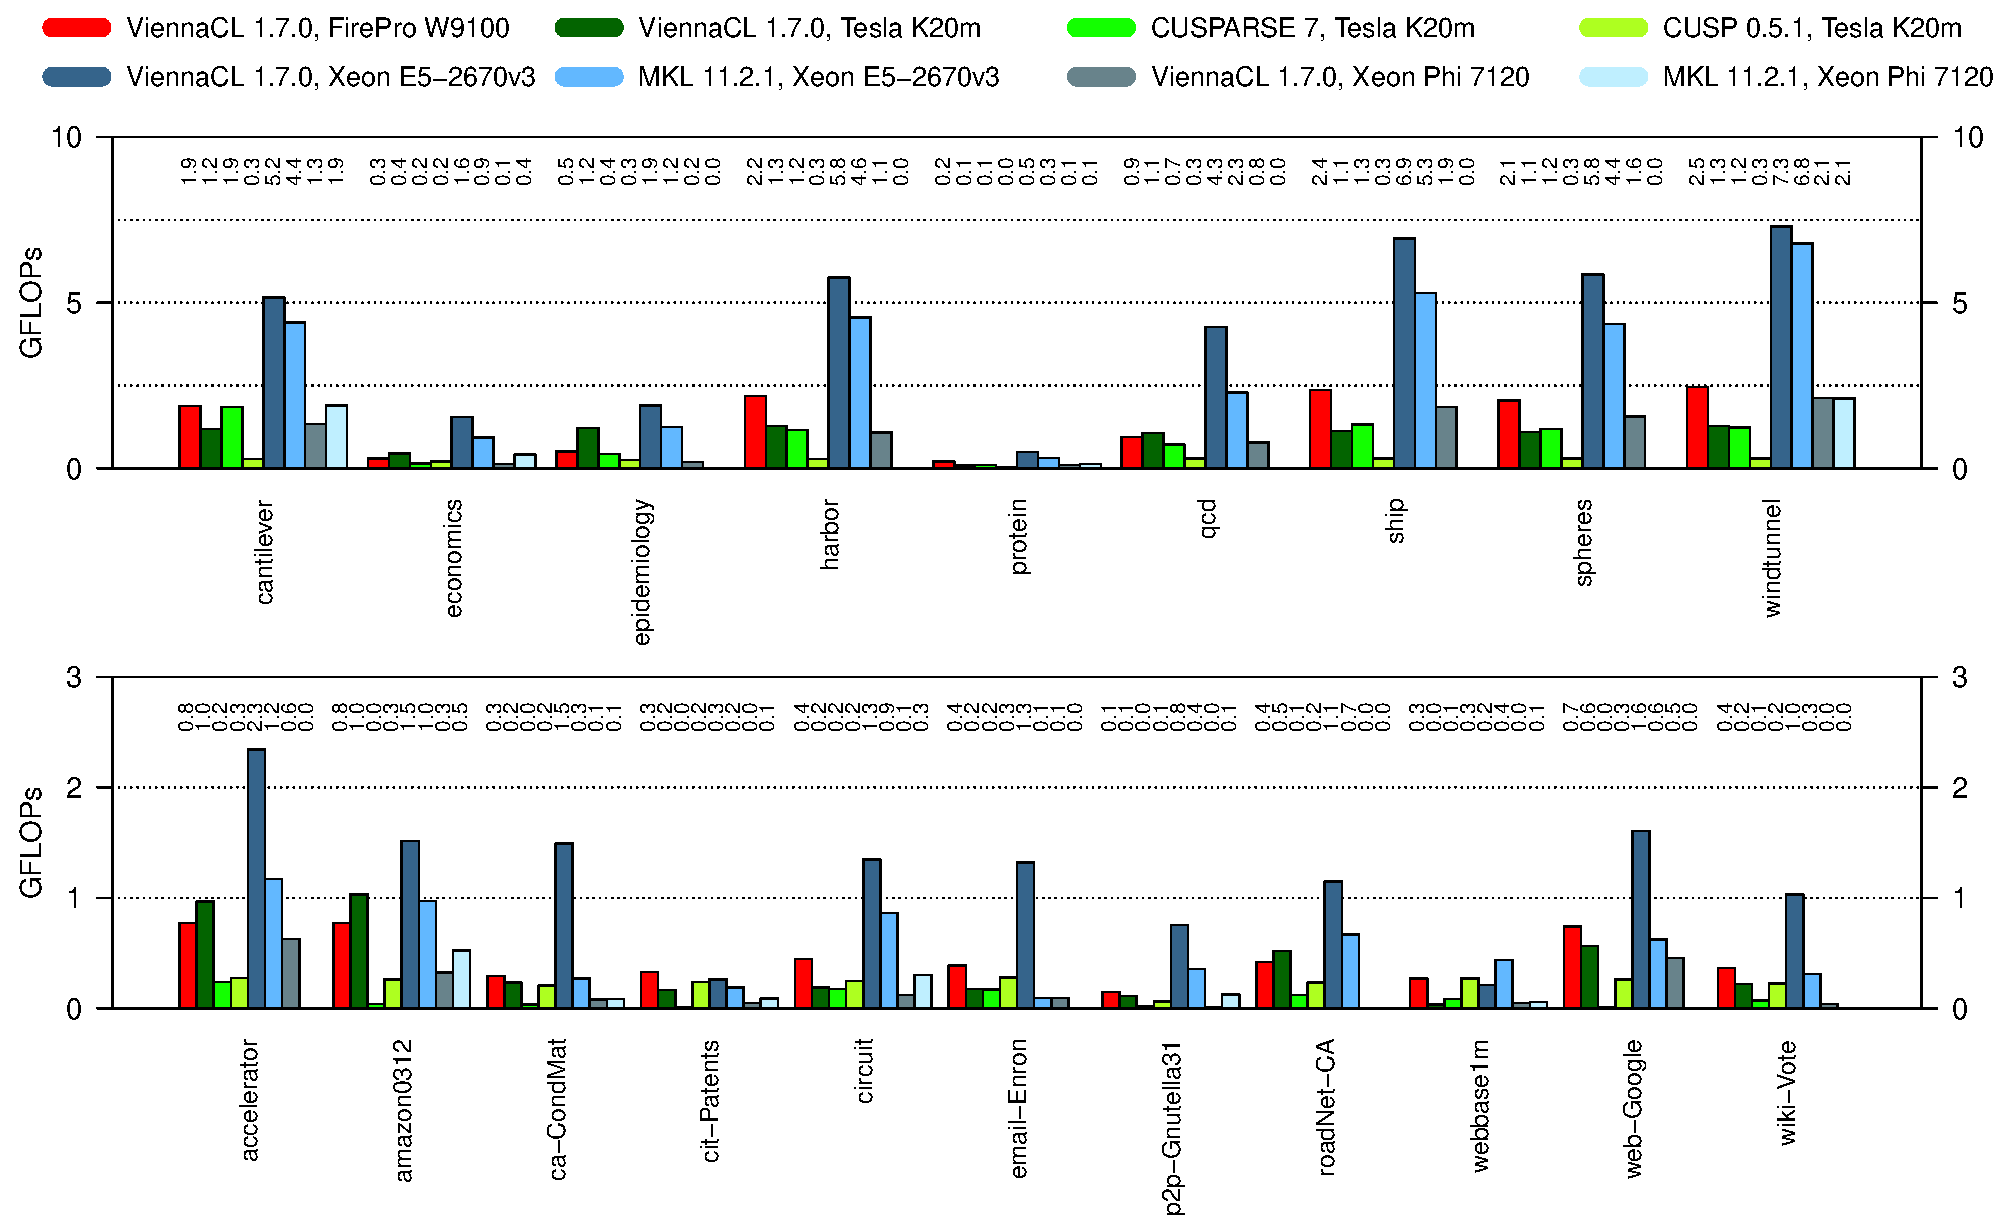
\includegraphics[width=1.05\textwidth]{figures/spgemm}
   \end{center}
  \end{block}
\end{frame}


% AMG
\begin{frame}{Upcoming PETSc+ViennaCL Feature}
  \begin{block}{Algebraic Multigrid Preconditioners}
  \vspace*{-.2cm}
   \begin{center}
    \includegraphics[width=0.9\textwidth]{figures/amg-vs-pure-full-2d}
   \end{center}
  \end{block}
\end{frame}


% Parallel ILU
\begin{frame}{Pipelined Solvers}
  \begin{block}{Fine-Grained Parallel ILU (Chow and Patel, SISC, 2015)}
  \vspace*{-.2cm}
   \begin{center}
    \includegraphics[width=0.9\textwidth]{figures/ilu-3d}
   \end{center}
  \end{block}
\end{frame}

